\chapter{Regression}
\label{ch:capitolo4}
Different regression techniques were applied to the dataset, testing
on different combinations of attributes. The target variable chosen for
Univariate and Multiple regression was \texttt{criticReviewsTotal}, while
for Multivariate regression, the target variables were both
\texttt{userReviewsTotal} and \texttt{criticReviewsTotal}.
These were chosen because they offer important insights into the engagement
that a product can generate, which also was the focus of the binary
classification task in section~\ref{sec:binary_classification}.


\section{Univariate and Multiple Regression}
For Univariate Regression, the attribute
\texttt{criticReviewsTotal} was chosen
as the target variable. Aside from the semantic meaning, this choice was also made
because it has a high correlation
with the attribute \texttt{userReviewsTotal}, allowing univariate regression
to be performed, while maintaining a clear separate semantic meaning.
% Figure~\ref{fig:univariate_regression} shows the results of the Univariate Regression task for
% all models but KNN, which doesn't provide an interesting visualization.
% \begin{figure}[H]
%     \centering
%     \begin{subfigure}{0.2565\textwidth}
%         \centering
%         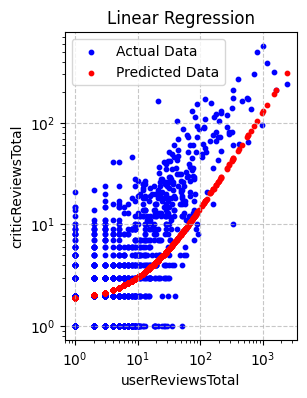
\includegraphics[width=1\textwidth]{plots/linear.png}
%         \caption{Linear regressor}
%         \captionsetup{width=0.9\linewidth, justification=centering}
%         \label{fig:linear}
%     \end{subfigure}
%     \begin{subfigure}{0.24\textwidth}
%         \centering
%         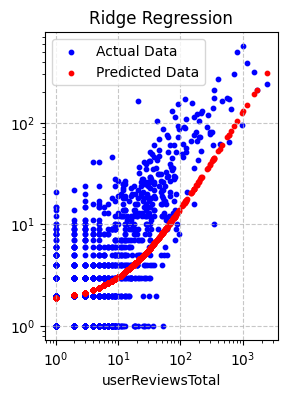
\includegraphics[width=1\textwidth]{plots/ridge.png}
%         \caption{Ridge regressor}
%         \captionsetup{width=0.9\linewidth, justification=centering}
%         \label{fig:ridge}
%     \end{subfigure}
%     \begin{subfigure}{0.24\textwidth}
%         \centering
%         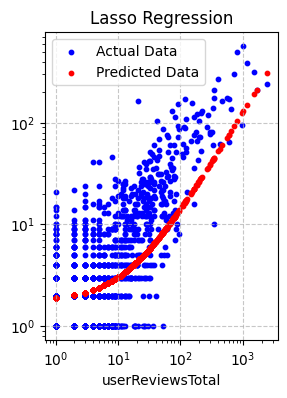
\includegraphics[width=1\textwidth]{plots/lasso.png}
%         \caption{Lasso regressor}
%         \captionsetup{width=0.9\linewidth, justification=centering}
%         \label{fig:lasso}
%     \end{subfigure}
%     \begin{subfigure}{0.24\textwidth}
%         \centering
%         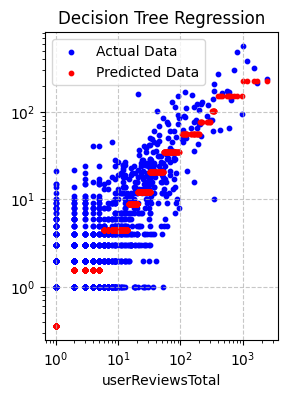
\includegraphics[width=1\textwidth]{plots/dt_regressor.png}
%         \caption{DT regressor}
%         \captionsetup{width=0.9\linewidth, justification=centering}
%         \label{fig:elastic}
%     \end{subfigure}
%     \caption{Univariate regression prediction results in Logarithmic space}
%     \label{fig:univariate_regression}
% \end{figure}

\begin{table}[H]
    \centering
    \begin{tabular}{lccccccc}
        \toprule
        % mae, mse normalized over target variable range
         & \textbf{Intercept} & \textbf{Coefficient} & \textbf{R$^2$} & \textbf{MAE} & \textbf{MSE} & \textbf{$\alpha$} \\
        \midrule
        \textbf{Univariate} \\
        \midrule
        Linear & 1.760 & 0.126 & 0.357 & 0.007 & 0.334 & - \\
        Ridge & 1.760 & 0.126 & 0.357 & 0.007 & 0.334 & 100 \\ % alpha=100
        Lasso & 1.924 & 0.100 & 0.342 & 0.006 & 0.376 & 100 \\ % alpha=100
        DT & - & - & 0.678 & 0.004 & 0.194 & - \\
        24-NN & - & - & 0.658 & 0.004 & 0.223 & - \\
        \midrule
        \textbf{Multiple}\\
        \midrule
        Linear & - & - & 0.601 & 0.006 & 0.220 & - \\
        Ridge & - & - & 0.601 & 0.006 & 0.220 & 0.1 \\ % alpha=0.1
        Lasso & - & - & 0.590 & 0.005 & 0.241 & 1 \\ % alpha=1
        DT & - & - & 0.784 & 0.004 & 0.196 & - \\
        7-NN & - & - & $\approx 1$ & 0.003 & 0.176 & - \\
        \bottomrule
    \end{tabular}
    \caption{Classification report for binary classification}
    \label{tab:binary_classification_report}
\end{table}
% \begin{table}[H]
%     \centering
%     \begin{tabular}{lccccccccc}
%         \toprule
%         % mae, mse normalized over target variable range
%          & \textbf{Intercept} & \textbf{Coefficient} & \textbf{MAE} & \textbf{MSE} & \textbf{R$^2$} & \textbf{test MAE} & \textbf{test MSE} & \textbf{$\alpha$} \\
%         \midrule
%         \textbf{Univariate} & & & & & \\
%         \midrule
%         Linear & 1.760 & 0.126 & 0.007 & 0.253 & 0.357 & 0.007 & 0.334 & - \\
%         Ridge & 1.760 & 0.126 & 0.007 & 0.253 & 0.357 & 0.007 & 0.334 & 100 \\ % alpha=100
%         Lasso & 1.924 & 0.100 & 0.007 & 0.259 & 0.342 & 0.006 & 0.376 & 100 \\ % alpha=100
%         DT & - & - & 0.005 & 0.127 & 0.678 & 0.004 & 0.194 & - \\
%         24-NN & - & - & 0.004 & 0.135 & 0.658 & 0.004 & 0.223 & - \\
%         \midrule
%         \textbf{Multiple} & & & & & \\
%         \midrule
%         Linear & - & - & 0.006 & 0.157 & 0.601 & 0.006 & 0.220 & - \\
%         Ridge & - & - & 0.006 & 0.157 & 0.601 & 0.006 & 0.220 & 0.1 \\ % alpha=0.1
%         Lasso & - & - & 0.006 & 0.161 & 0.590 & 0.005 & 0.241 & 1 \\ % alpha=1
%         DT & - & - & 0.004 & 0.085 & 0.784 & 0.004 & 0.196 & - \\
%         7-NN & - & - & $7 * 10^{-5}$ & $8 * 10^{-5}$ & $\approx 1$ & 0.003 & 0.176 & - \\
%         \bottomrule
%     \end{tabular}
%     \caption{Classification report for binary classification}
%     \label{tab:binary_classification_report}
% \end{table}
While Linear, Ridge and Lasso's predictions are similar in both 

For Multiple Regression, the target variable was kept the same, in order to
allow for a direct comparison of the results obtained with the two techniques.


\section{Multivariate Regression}
